\documentclass{article}
\usepackage[utf8]{inputenc}
\usepackage{geometry}
\usepackage{amsmath}
\usepackage{dirtytalk}
\usepackage{graphicx}
\usepackage{enumerate}
\usepackage{hyperref}
\usepackage{listings}
\usepackage{multicol}

\setlength\columnsep{30pt}

\geometry{
 	a4paper,
	total={170mm,257mm},
 	left=20mm,
 	top=20mm,
}

\lstset{basicstyle=\footnotesize\ttfamily,breaklines=true}

\title{
	 \large 518: Logic and AI Programming \\
	 \huge Prolog Reference
}
\date{7 Jan 2018}
\author{
	Sam Yong \\
	\small \href{mailto:sam.yong17@imperial.ac.uk}{sam.yong17@imperial.ac.uk}
}


\begin{document}
  \maketitle
  
  \begin{multicols}{2}
  
  \section*{Foreword}  
  
  \paragraph{} This Prolog reference was made as an condensation from the lecture slides and notes provided by Dr Fariba Sadri, Claudia Schulz and Romain Barnoud in the Imperial College London, Department of Computing's 518: Logic and AI Programming course.
  
  \paragraph{} This reference also contain several contributions\footnote{List of contributors in no particular order.} by Aaron Hau and Sagar Doshi. Thank you!
  
  \paragraph{} The ordering of this reference may not correspond to the sequence introduced in the lectures, lecture slides and notes. This order is how I feel I would understand the topic better.
  
  \begin{footnotesize}
  \paragraph{License} This reference is made publicly available under the MIT License. You should not have paid anyone money in exchange for this document. If you have paid someone for it, well too bad. The source code for this document can be found public available on my Github repository\footnote{\href{https://github.com/mauris/written}{https://github.com/mauris/written}}. If you wish to help improve this document, feel free to open an issue on the Github repository.
  \end{footnotesize}
  
  \tableofcontents
  
  \newpage
  
  \section{Introduction to Prolog}
  
  \subsection{Syntax}
  
  \subsubsection{Clauses}
  
  \paragraph{Prolog programs} are sequences of clauses. Clauses can be:
  
  \begin{enumerate}
  \item Conditional Clause: $H :- C_1, C_2, ..., C_k.$; or,
  \item Unconditional Clause $H.$
  \end{enumerate}
  
  \noindent Notice that clauses need to terminate with "$.$". If an unconditional clause contains no variables, the clause can also be called a {\bf fact} while all other Prolog clauses are called {\bf rules}. $\forall i\ C_i$ are also known as {\bf conditions} of the clause. $H$ and $\forall i\ C_i$ are each an atomic formula in the form:
  
  $p(t_1, t_2, ... t_n)$ or $p$
  
  \noindent There must be no space between "$p$" and the open parenthesis "$($".
  
  The clause $H :- C_1, C_2, ..., C_k.$ can also be read as $\forall X_1, ... X_m (C_1 \land ... \land C_k \implies H)$ in predicate logic. $H$ only holds if $\forall i C_i$ conditions hold.
  
  \paragraph{Commas} are considered as conjunction (AND operator) in a Prolog statement as mentioned in the previous paragraph.
  
  \paragraph{Semi-colons} To represent disjunction (OR operator) in bodies of rules, the semi-colon "$;$" symbol can be used as such:
  
  \begin{lstlisting}
  has_jam(R) :-
    has_road_works(R);
    has_car_accident(R).
  \end{lstlisting}
  
  Disjunction in rules can also be broken into separate clauses. The clause above can be also written as:
  
  \begin{lstlisting}
  has_jam(R) :-
    has_road_works(R).
  has_jam(R) :-
    has_car_accident(R).
  \end{lstlisting}
  
  \paragraph{Negation} To negate a condition, the expression "$\backslash+$" is used before the condition. For example:
  
  \begin{lstlisting}
  can_buy_alcohol(P) :-
    \+ underage(P).
  \end{lstlisting}
  
  \noindent is read as "P can buy alcohol if P is {\bf not} underage." Multiple clauses can also be negated by using $()$ parentheses: 
  
  \begin{lstlisting}
  road_is_clear(R) :-
    \+ (has_road_works(R);
      has_car_accident(R)).
  \end{lstlisting}
  
  \subsubsection{Anonymous Variables} 
  
  \paragraph{} Variables that only appear once in a rule can be made {\bf anonymous}, i.e. they do not have to be named in the rule. An underscore "$\_$" can be used in place of such variables, for example:
  
  \begin{lstlisting}
  needs(_, computers).
  \end{lstlisting}
  
  Two or more underscores in the same rule are used to represent different variables, for example:
  
  \begin{lstlisting}
  happy(S) :-
    likes(_, logic),
    likes(_, _prolog).
  \end{lstlisting}
  
  \noindent is understood as:
  
  \begin{lstlisting}
  happy(S) :-
    likes(X, logic),
    likes(Y, _prolog).
  \end{lstlisting}
  
  \subsubsection{Prolog Terms}
  
  \paragraph{A Prolog term} is one of the following:
  
  \begin{enumerate}
  \item Atom/Constant: starts with a lower-case letter or anything between quotes. e.g.: \textit{john, computing\_MSc, x123, 'logic and ai'.}
  \item Number: an integer or float. e.g.: \textit{0, 42, -1729, 2.718, 6.626E-34}
  \item Variable: starts with a upper-case letter or an underscore. e.g.: \textit{My\_variable, X, \_Anonymous, \_123, \_} 
  \item Compound Term\footnote{Note that they are terms, not functions}: in the form of $functor(t_1,..., t_n)$, where $functor$ is a constant name applied to $n$ terms. $n$ is called the arity of the term.\footnote{Constants are 0-arity terms}. e.g.: \textit{dob(alice, 1970), world\_record('100m', 9.58, date(16, august, 2009)), 'long name here'(X, cst, \_)}
  \end{enumerate}
  
  \noindent A {\bf ground term} is a term that contains no variable. For example:
  
  \begin{lstlisting}
  has_plant(kelvin, ginger)
  age(james, 20)
  \end{lstlisting}
  
  \subsubsection{Comments}
  
  \paragraph{} Comments can be written in a Prolog file by using the $\%$ character at the beginning of the comment. All characters following the $\%$ character until the newline character are ignored by Prolog. For example:
  
  \begin{lstlisting}
  % this is a prolog comment
  happy(sarah).
  \end{lstlisting}
  
  \subsection{Execution Modes}  
  
  \paragraph{} Prolog\footnote{There are several implementations of Prolog, such as Sicstus and SWI Prolog.} is a console / terminal program that acts takes in the sequences of clauses in sequence of prompt and result. When Prolog starts, the program will show a prompt like this: \vspace{0.3cm}
  
  \noindent 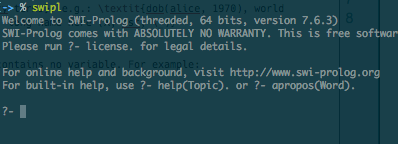
\includegraphics[scale=0.55]{terminal.png}
  
  \paragraph{} The prompt shows as "$?-$" and you can enter Prolog clauses at the prompt. To exit Prolog, use the $halt/0$ built-in predicate by typing in "$halt.$" to exit.
  
  \paragraph{} Since there is a need to distinguish between fact clauses for the execution environment and query clauses, Prolog offers another built-in predicate $consult/1$ for this purpose. There are two ways to enter facts into the current Prolog environment:
  
  \begin{enumerate}
  \item \lstinline{consult(user).} or \lstinline{[user].} - Changes the prompt into facts input mode. When in this mode, you can directly enter fact clauses. When done, enter the EOF character (usually Ctrl+D) and Prolog will go back to the query mode.
  \item \lstinline{consult('filename.pl').} - Load facts from a file named "filename.pl" (you can change this to another name of a file that exists on the file system). The fact clauses can be saved as a file in plain text and loaded in this way.
  \end{enumerate}
  
  \paragraph{Listing} To view all currently loaded predicates, you can use $listing/0$. The $listing/1$, where it is defined as \lstinline{listing(Predicate/n).} predicate can be used to show all definitions of \lstinline{Predicate} with $n$ terms.
  
  \paragraph{Saving to file} To save your listing as a file, you can use the following query clauses:
  
  \begin{lstlisting}
  ?- tell('filename.pl').
  ?- listing.
  ?- told.
  \end{lstlisting}
  
  \subsection{Getting out}
  
  \paragraph{} If you were to write a program like this:
  
  \begin{lstlisting}
  stuck(_) :- stuck(_).
  \end{lstlisting}
  
  \noindent ... and if you run the query:
  
  \begin{lstlisting}
  ?- stuck(a).
  \end{lstlisting}
  
  \noindent You'll find that Prolog gets stuck at the query because of an infinite loop. To pause the query execution, press the "Ctrl+C" key and Prolog will then show a prompt asking for the next course of action. Pressing "h" will show the full menu and "a" to abort the execution.
  
  \begin{lstlisting}
  ?- stuck(a).
  ^CAction (h for help) ? Options:
  a:       abort      b:      break
  c:       continue   e:      exit
  g:       goals      s:      C-backtrace
  t:       trace      p:      Show PID
  h (?):   help
  Action (h for help) ? 
  \end{lstlisting}

  \subsection{Test and Generate}
  
  There are two ways to use goals in Prolog. You can either test to verify a fact or generate to yield possible variables that apply to the goals. For example, a test is written such as:
  
  \begin{lstlisting}
  ?- permutation([1, 3, 2], [3, 2, 1]).
  true.
  \end{lstlisting}
  
  In tests, Prolog does nothing more than returning true when the query succeed and false when the query fail. A generate is written as such:
  
  \begin{lstlisting}
  ?- remove(3, [1, 3, 2], L).
  L = [1, 2].
  \end{lstlisting}
  
  In generate, all sets of non-variable terms that substitute all variables in the query to satisfy the query are printed.
  
  \subsection{Declarative vs Procedural}
  
  \paragraph{Consider the rule $A :- B, C.$} The declarative meaning\footnote{or logical interpretation} is $A \impliedby B \land C$, which means A is true if B is true and C is true. However, how Prolog interprets the rule\footnote{i.e. procedural meaning} is to first prove $A$, prove $B$, and then prove $C$ in that specific order. 
  
  \paragraph{Now, consider the rule $A :- B.\ A :- C.$} The declarative meaning is $A \impliedby B \lor C$, which means $A$ is true if $B$ is true or $C$ is true. However, how Prolog interprets the rule is to first prove $B$ to prove $A$. If $B$ does not succeed, then prove $C$ to prove $A$. 
  
  \paragraph{Lastly, consider $p :- p.$} The declarative meaning is $p \impliedby p$, which by definition is a tautology. However, how Prolog interprets the rule is to prove $p$, prove $p$, ...  which causes an infinite loop.
  
  \subsection{Predicate Signature}
  
  \paragraph{Predicate Signature} Like a function signature, the predicate signature tells which parameters are expected and what kind of parameters are expected for the predicates. In particular:
  
  \begin{enumerate}[\hspace{1.4cm}]
  \item[\bf +Arg1:] $Arg1$ is expected {\bf not} to be a variable (but may contain variables).
  \item[\bf -Arg2:] $Arg2$ is expected to be a variable.
  \item[\bf ?Arg3:] No assumptions is made on whether $Arg3$ is a variable or not.
  \end{enumerate}
  
  \subsection{Debugging}
  
  \paragraph{} Debugging in the Prolog query environment can be done using the $trace.$ and $notrace.$ terms. To start tracing how a query is answered, type and enter:
  
  \begin{lstlisting}
  ?- trace.
  \end{lstlisting}
  
  Notice that the prompt changes from $?-$ to $[trace]  ?-$ which indicates that you are now in trace mode. Any subsequent queries except $notrace$ will be executed with each step of the search strategy shown. To turn off tracing, type and enter:
  
  \begin{lstlisting}
  [trace]  ?- notrace.
  \end{lstlisting}
  
  \section{Substitution}
  
  \paragraph{Definition} A substitution is a mapping from variables to terms, as such:
  
  $$\theta = \{ X_1 \mapsto t_1, X_2 \mapsto t_2, ..., X_n \mapsto t_n \}$$
  
  When a substitution $\theta$ is applied to a term $t$, it is written $s = t\theta$, where the new term $s$ is identical to $t$ with $\forall i \in [1, n]$, $X_i$ is replaced with $t_i$. $s$ is called an instance of $t$.
  
  \paragraph{Examples} Some examples of substitution are:
  
  \begin{enumerate}
  \item $t = f(A,B),\\ \theta = \{A \mapsto x, B \mapsto y\}$\\ gives $s=t\theta=f(x, y)$
  \item $t = g(X, f(c, X), Y),\\ \theta = \{X \mapsto a, Y \mapsto Z\}$\\ gives $s=t\theta=g(a, f(c, a), z)$
  \item $t = h(X, Y, Z),\\ \theta = \{X \mapsto W, Y \mapsto f(W), Z \mapsto f(b)\}$\\ gives $s=t\theta=h(W, f(W), f(b))$
  \end{enumerate}
  
  \section{Unification}
  
  \paragraph{Definition} Two terms $T_1$ and $T_2$ unify iff $\exists$ a subtitution $\theta$ s.t. $T_1\theta \equiv T_2\theta$.
  
  \paragraph{Examples} Some examples of unification are:
  
  \begin{enumerate}
  \item $john$ unifies with $john$, iff $\theta = \{\}$.
  \item $alice$ unifies with $Alice$, iff $\theta = \{Alice \mapsto alice\}$. Recall that $Alice$, having a upper-case first letter, is a variable.
  \item $\_000$ unifies with $Variable$, iff $\theta = \{\_000 \mapsto Variable\}$ or $\theta = \{Variable \mapsto \_000\}$.
  \item $p(X, 2)$ unifies with $p(f(g), Y)$, iff $\theta = \{X \mapsto f(g), Y \mapsto 2\}$. Recall that $\theta$ needs to be applied to both terms.
  \item $p(X, f(Y))$ unifies with $p(f(f(b)), X)$, iff $\theta = \{X \mapsto f(f(b)), Y \mapsto f(b)\}$.
  \end{enumerate}
  
  The following are some examples of non-unification:
  
  \begin{enumerate}
  \item $3$ does not unify with $3.0$.
  \item $518$ does not unify with $'518'$. Recall that $'518'$ is an atom/constant term while $518$ (without quotes) is a number term.
  \item $g(a, b, c)$ does not unify with $h(a, b, c)$. $g$ and $h$, being compound terms cannot be substituted\footnote{Only variables can be substituted}.
  \item $f(a, X)$ does not unify with $f(X, b)$. The variable $X$ cannot be mapped to two different terms.
  \item $p(X, f(Y))$ does not unify with $p(a, X)$. Like previous example, $X$ cannot be mapped to $a$ and $f(Y)$ at the same time.
  \end{enumerate}
  
  \section{Comparison \& Equality}
  
  \paragraph{} There are four equality predicates in Prolog: $=$, $==$, $is$ and $=:=$. Suppose $S$, $T$ and $X$ are terms and Expr, Expr1, Expr2 are arithmetic expressions, the following statements hold:
  
  \begin{enumerate}
  \item $S = T$ iff $S$ and $T$ unify.
  \item $S == T$ iff $S$ and $T$ are identical.
  \item $X is Expr$ iff the result of evaluating $Expr$ unifies with $X$.
  \item $Expr1 =:= Expr2$ iff $Expr1$ and $Expr2$ both evaluate to the {\bf same number}.
  \end{enumerate}
  
  \paragraph{Inequality} The following are the opposite predicates for the four equality predicates:
  
  \begin{enumerate}
  \item The negation of $=$ is $\backslash=$.
  \item The negation of $==$ is $\backslash==$.
  \item The negation of $is$ is undefined.
  \item The negation of $=:=$ is $=\backslash=$.
  \end{enumerate}
  
  \paragraph{Standard Order of Terms} There's a standard ordering of terms, which is defined as:
  
  \noindent \small Variables\textless Floats\textless Integers\textless Atoms\textless Compound Terms
  
  Variables are sorted by their appearances; Numbers are compared according to their natural order (but floats are always smaller than integers\footnote{SWI Prolog uses a different system for ordering numbers. See \href{http://www.swi-prolog.org/pldoc/man?section=compare}{http://www.swi-prolog.org/pldoc/man?section=compare}}); Atoms are compared to atoms alphabetically; and, Compound terms are compared by: their arity, then functor name alphabetically, then recursively their arguments from left to right. 
  
  Term comparisons can be done using the following:
  
  \begin{enumerate}
  \item \lstinline{P == Q} to check if two terms are of equal order.
  \item \lstinline{P \== Q} to check if two terms are of unequal order.
  \item \lstinline{P @< Q} to check if term $P$ is of order less than $Q$.
  \item \lstinline{P @=< Q} to check if term $P$ is of order less than or equal to $Q$.
  \item \lstinline{P @> Q} to check if term $P$ is of order more than $Q$.
  \item \lstinline{P @>= Q} to check if term $P$ is of order more than or equal to $Q$.
  \end{enumerate}
  
  Alternatively, the built-in $compare/3$ predicate can be used.
  
  \section{Search Strategy}
  
  \paragraph{Query} A query is a conjunction of goals \lstinline{G1, G2, ..., Gn} written as such:
  
  \begin{lstlisting}
  ?- G1, G2, ..., Gn.
  \end{lstlisting}
  
  \paragraph{Answer} An answer to a query is one substitution $\theta$ s.t. $G1\theta, G2\theta, ..., Gn\theta$ are the logical consequences of the program.
  
  Prolog uses a search strategy find one such substitution or prove that such substitution does not exist.
  
  \subsection{Algorithm}
  
  \paragraph{} To solve a given query $?- G1, G2, ..., Gn.$
  
  \begin{enumerate}
  \item Start with solving first goal $G1$.
  \item To solve $G1$, find a fact / clause $H := B1, B2, ..., Bm$ where $H$ unifies with $G1$ (i.e. $\exists\theta, G1\theta \equiv H\theta$). If there are more than one clause that satisfies the above condition, we have reached a choice point: select potential clauses from top to bottom. 
  \begin{enumerate}
  \item If $G1$ is the only goal in the query (i.e. $n=1$) and the selected clause is a fact (i.e. $H.$, $m=0$). {\bf $\implies$ succeed}
  \item - If such a clause and substitution exist, extend and solve the query "$?- B1\theta, B2\theta, ..., Bm\theta, G2\theta, ..., Gn\theta.$".
  \item - If no such clause or substitution exists, {\bf backtrack} to the last choice point and pick next satisfiable clause.
  \item If there are no more choice points (i.e. all clauses for all choice points have been tried), {\bf $\implies$ fail}
  \end{enumerate}
  \end{enumerate}
  
  \paragraph{Search Tree} A search tree can be used to visualize the steps that the Prolog search strategy algorithm takes when answering queries.
  
  \begin{enumerate}
  \item At each step, the applicable clauses represent alternative evaluation paths (different branches of the search tree).
  \item Prolog searches the tree left-to-right, depth-first, to find successful evaluation paths.
  \item If a leaf query has no applicable clause, the path/branch of the search tree fails.
  \item If a leaf query is an empty conjunction, the path/branch of the search tree succeeds.
  \end{enumerate}
  
  \section{Recursion}
  
  \paragraph{Definition} A {\bf recursive} predicate is a predicate that calls itself. For example:
  
  \begin{lstlisting}
  recursive_predicate(X1, ..., Xn) :-
    goal1,
    ...
    goalP,
    recursive_predicate(Y1, ..., Yn),
    goalQ,
    ...,
    goalR.
  \end{lstlisting}
  
  \paragraph{Tail Recursion} A recursive predicate is {\bf tail recursive} iff the recursion occurs in the last goal of each recursive rule. 
  
  \paragraph{Base Case(s)} Recursions need at least one base case so that the algorithm knows when to terminate the recursion and backtrack. The base case(s) is/are usually placed before the recursion case(s).
  
  \subsection{Loops}
  
  Loops do not exist in Prolog as Prolog is primarily a declarative language rather than procedural (like C++). However, recursion can be used to replace loops as such:
  
  \begin{lstlisting}
  while_loop(I, N, X1, ...) :-
    I =:= N,
    % end of the loop.
  
  while_loop(I, N, X1, ...) :-
    I < N,
    % do work in loop
    NewI is I+1,
    while_loop(NewI, N, Y1, ...).
  \end{lstlisting}
  
  \subsection{Examples}  
  
  \paragraph{factorial/2} Calculate the factorial $f(n) = n!$:
  
  \begin{lstlisting}
  factorial(?N, ?Result)
  \end{lstlisting} 
  
  Returns $true$ if $Result$ unifies with the factorial of $N$, $false$ otherwise. $factorial/2$ can be defined as follows:
  
  \begin{lstlisting}
  factorial(0, 1).
  factorial(F, FN) :-
    N > 0,
    M is N-1,
    factorial(M, FM),
    FN is N*FM.
  \end{lstlisting}
  
  \section{Lists}  
  
  \subsection{Introduction}
  
  \paragraph{} Lists are useful to represent sequences or collection of things. For example, instead of writing multiple predicates as such:
  
  \begin{lstlisting}
  dept(eng, aero).
  dept(eng, bio_eng).
  dept(eng, computing).
  dept(eng, eee).
  dept(eng, mech_eng).
  dept(sci, chemistry).
  dept(sci, maths).
  dept(sci, physics).
  dept(business, finance).
  dept(business, management).
  \end{lstlisting}
  
  the predicates can be simplified by changing them to:
  
  \begin{lstlisting}
  dept(eng, [aero, bio_eng, computing,
   eee, mech_eng]).
  dept(sci, [chemistry, maths, physics]).
  dept(business, [finance, management]).
  \end{lstlisting}
  
  As you may notice, you no longer can test for facts by performing for example $dept(sci, maths).$ because the facts are represented in list. To test for the facts, it is possible to add an additional predicate as such:

  \begin{lstlisting}
  dept(X, Y) :-
    dept(X, L),
    member(Y, L).
  \end{lstlisting}
  
  and you will be able to test if the fact was stated using the statement:

  \begin{lstlisting}
  ?- dept(eng, aero).
  \end{lstlisting}
  
  In Prolog, elements in a list can be any Prolog terms, including a list. For example $[a, 1, f(X, Y), [4, Z, 6], 2.0]$ is a valid Prolog expression representing a list.
  
  \subsection{Definition}
  
  \say{A list is a data structure that represents a sequence of any number of terms.} - Wisdom.
  
  \paragraph{} A Prolog list is one of the following:
  
  \begin{enumerate}
  \item $[]$ - an empty list; or,
  \item $[H|T]$ - where $H$ is a term and $T$ is a list (recursive definition). $H$ being the first item of the list is called the {\bf head} and $T$ being the remaining of the list is called the {\bf tail}.
  \end{enumerate}
  
  \noindent The following expressions are equivalent:
  
  \begin{equation*}
  \begin{aligned}
  \big [ a \vert [ b \vert [ c \vert [ d \vert []]]] \big] & \equiv [a,b,c,d] \\
  & \equiv [a|[b,c,d]] \\
  & \equiv [a,b|[c,d]] \\
  & \equiv [a,b,c|[d]] \\
  & \equiv [a,b,c,d|[]]
  \end{aligned}
  \end{equation*}  
  
  \noindent Note that the empty list $[]$ has an undefined head and an undefined tail.  
  
  \subsection{Lists Library}
  
  \paragraph{} Prolog provides some built-in predicates for manipulating lists via the "lists" library. \footnote{Documentation available at \url{https://sicstus.sics.se/sicstus/docs/4.3.0/html/sicstus/lib_002dlists.html}}
  
  \paragraph{} To load the library, you can either use the query:
  
  \begin{lstlisting}
  ?- use_module(library(lists)).
  \end{lstlisting}
  
  or add the following rule to your program:

  \begin{lstlisting}
  :- use_module(library(lists)).
  \end{lstlisting}
  
  \subsection{Built-in Lists Predicates}
  
  \subsubsection{Membership}
  
  \paragraph{member/2} Test if an element is in a list:
  
  \begin{lstlisting}
  member(?Element, ?List)
  \end{lstlisting} 
  
  Returns $true$ if $Element$ occurs in $List$, $false$ otherwise.

  \paragraph{nonmember/2} Test if an element is not in a list:
  
  \begin{lstlisting}
  nonmember(?Element, ?List)
  \end{lstlisting} 
  
 Returns $true$ if $Element$ does not occur in $List$, $false$ otherwise.
  
  \subsubsection{List Operations}

  \paragraph{append/3} Test if an element is not in a list:  
  
  \begin{lstlisting}
  append(?List1, ?List2, ?List3)
  \end{lstlisting} 
  
  Returns $true$ if $List3$ is the list consisting of $List1$ followed by $List2$, $false$ otherwise.
  
  \paragraph{length/2} Test if a list is of a certain length:
  
  \begin{lstlisting}
  length(?List, ?Length)
  \end{lstlisting} 
  
  Returns $true$ if $List$ contains $Length$ number of elements, $false$ otherwise.
  
  \paragraph{rev/2} Test if a two lists are the reverse of each other:
  
  \begin{lstlisting}
  rev(+List, ?Reversed)
  \end{lstlisting} 
  
  Returns $true$ if $List$ and $Reversed$ contain the same elements but in reverse order, $false$ otherwise.
  
  The $rev/2$ predicate can also be easily defined in direct recursion or using accumulator. The following is an implementation of $rev/2$ using direct recursion:
  
  \begin{lstlisting}
  rev2([], []).
  rev2([H|T], R) :-
    rev2(T, RT),
    append(RT, [H], R).
  \end{lstlisting}
  
  The following is then an implementation of $rev/2$ using an accumulator:
  
  \begin{lstlisting}
  rev3(L, RL) :-
    rev_acc(L, [], RL).
  rev_acc([], Acc, Acc).
  rev_acc([H|T], Acc, RL) :-
    rev_acc(T, [H|Acc], RL).
  \end{lstlisting}
  
  \paragraph{sort/2} Sorts a list:\footnote{See it. Say it. Sorted. - TfL}
  
  \begin{lstlisting}
  sort(+List, -Sorted)
  \end{lstlisting} 
  
  Elements from $List$ are sorted in ascending order and duplicated elements are removed. The resulting list is unified with $Sorted$.
  
  \paragraph{perm/2} Test if a two lists are the permutations of each other:
  
  \begin{lstlisting}
  perm(+List, -Perm)
  \end{lstlisting} 
  
  Returns $true$ if $List$ and $Perm$ are permutations of each other, $false$ otherwise.
  
  \paragraph{subseq0/2} Test if a list is a sub-sequence of another:
  
  \begin{lstlisting}
  subseq0(+Seq, -SubSeq)
  \end{lstlisting} 
  
  Returns $true$ if $SubSeq$ is a sub-sequence of $Seq$, $false$ otherwise.
  
  \subsection{User-Defined Predicates}

  \paragraph{belongs\_to/2}: Test if an element belongs to a list:
  
  \begin{lstlisting}
  belongs_to(?Element, ?List)
  \end{lstlisting} 
  
  Returns $true$ if $List$ contains the element $Element$, $false$ otherwise. $belongs_to/2$ can be defined as follows:

  \begin{lstlisting}
  belongs_to(X, L) :-
      L = [X|_].
  belongs_to(X, L) :-
      L = [_|T],
      belongs_to(X, T).
  \end{lstlisting} 
  
  We can get a more concise expression by simplifying the definition as such:

  \begin{lstlisting}
  belongs_to(X, [X|_]).
  belongs_to(X, [_|T]) :-
      belongs_to(X, T).
  \end{lstlisting} 
  
  \paragraph{concat/3} Concatenate two lists into the third:
  
  \begin{lstlisting}
  concat(?List1, ?List2, ?List3)
  \end{lstlisting} 
  
  $List1$ and $List2$ are concatenated together and returns $true$ if the resulting list is unified with $List3$, $false$ otherwise. $concat/3$ can be defined as follows:

  \begin{lstlisting}
  concat(L1, L2, L3) :-
      L1 = [], L3 = L2.
  concat(L1, L2, L3) :- 
      L1 = [H1|T1],
      concat(T1, L2, T3),
      L3 = [H1|T3].
  \end{lstlisting} 
  
  We can get a more concise expression by simplifying the definition as such:

  \begin{lstlisting}
  concat([], L, L).
  concat([H1|T1], L2, [H1|T3]) :- 
      concat(T1, L2, T3).
  \end{lstlisting}
  
  \paragraph{even\_odd/3} Partition a list into a list of its even elements and another list of its odd elements:
  
  \begin{lstlisting}
  even_odd(?List, ?Even, ?Odd)
  \end{lstlisting} 
  
  $List$ is partitioned into two lists $Even$ and $Odd$ where $Even$ contains all even numbered elements in $List$ and $Odd$ contains all odd numbered elements in $List$. $even_odd/3$ can be defined as follows:

  \begin{lstlisting}
  even_odd([], [], []).
  even_odd(L1, L2, L3) :- 
      L1 = [N|TList],
      N mod 2 =:= 0,
	  L2 = [N|TEven],
      even_odd(TList, TEven, L3).
  even_odd(L1, L2, L3) :- 
      L1 = [N|TList],
      N mod 2 =:= 1,
	  L3 = [N|TOdd],
      even_odd(TList, L2, TOdd).
  \end{lstlisting} 
  
  We can get a more concise expression by simplifying the definition as such:

  \begin{lstlisting}
  even_odd([], [], []).
  even_odd([N|TList], [N|TEven], L3) :- 
      N mod 2 =:= 0,
      even_odd(TList, TEven, L3).
  even_odd([N|TList], L2, [N|TOdd]) :- 
      N mod 2 =:= 1,
      even_odd(TList, L2, TOdd).
  \end{lstlisting} 
  
  \paragraph{last/2} Test if an element is the last element of a list:
  
  \begin{lstlisting}
  last(?Element, ?List)
  \end{lstlisting} 
  
  Returns $true$ if $Element$ is the last element of $List$, $false$ otherwise. $last/2$ can be defined as follows using the $append/2$:
  
  \begin{lstlisting}
  last(E, [E]).
  last(E, L) :-
      append(_, [E], L).
  \end{lstlisting} 
  
  $last/2$ can also be defined without using $append/2$ as follows:  
  
  \begin{lstlisting}
  last(E, [E]).
  last(E, [X,Y|L]) :-
      last(E, [Y|L]).
  \end{lstlisting} 
  
  \paragraph{len/2} While $length/2$ has been defined, it is still possible to test and generate the length of a list by writing some predicates. Test if an list is of a certain length:
  
  \begin{lstlisting}
  len(?List, ?Count)
  \end{lstlisting} 
  
  Returns $true$ if $List$ has $Count$ number of elements, $false$ otherwise. $len/2$ can be defined using {\bf direct recursion} as follows:
  
  \begin{lstlisting}
  len([], 0).
  len(L, N) :-
	L = [E|T],
	len(T, N1),
	N is N1+1.
  \end{lstlisting} 
  
  We can get a more concise expression by simplifying the definition as such:  
  
  \begin{lstlisting}
  len([], 0).
  len([_|T], N) :-
	len(T, N1),
	N is N1+1.
  \end{lstlisting} 

  If our goal is just to {\bf check} if the number of elements in the list equals to the $Count$ parameter, we can implement a faster solution $len2/2$ by writing it as such:
  
  \begin{lstlisting} 
  len2([], 0).
  len2([_|T], N) :-
    N1 is N-1,
  	len2(T, N1).
  \end{lstlisting}
  
  If you try to submit a query for a variable in the $Count$ parameter like $?- len2([1, 2, 3, 4, 5], N).$, Prolog will throw an error "Arguments are not sufficiently instantiated" because N is not instantiated.
  
  $len/2$ can also be implemented with an accumulator which improves the runtime performance:
  
  \begin{lstlisting} 
  len3(L, N) :- len_acc(L, 0, N).
  len_acc([], N, N).
  len_acc([E|T], CurrentN, N) :-
	NewN is CurrentN+1,
	len_acc(T, NewN, N).
  \end{lstlisting}  
  
  \paragraph{list\_double/2} Check if every element in a list is double of its corresponding element in another list.
  
  \begin{lstlisting}
  list_double(?List1, ?List2)
  \end{lstlisting} 
  
  Returns $true$ if every element in $List2$ is double of its corresponding element in $List1$. $list\_double/2$ can be defined as follows:

  \begin{lstlisting}
  list_double([E1], [E2]) :-
    E2 is E1*2.
  list_double([E1|T1], [E2|T2]) :-
    E2 is E1*2,
    list_double(T1, T2).
  \end{lstlisting} 
  
  \paragraph{sum/2} Calculate the sum of all elements in a list.
  
  \begin{lstlisting}
  sum(?List, ?Sum)
  \end{lstlisting} 
  
  Returns $true$ if summation of all elements in $List$ is equal to $Sum$. $sum/2$ can be defined using {\bf direct recursion} as follows:

  \begin{lstlisting}
  sum([], 0).
  sum([H|T], S) :-
    sum(T, N),
    S is H+N.
  \end{lstlisting} 
  
  However, using an accumulator would improve the performance of the summation:
  
  \begin{lstlisting}
  sum2(L, S) :- sum_acc(L, 0, S).
  sum_acc([], S, S).
  sum_acc([E|T], CurrentSum, Sum) :-
    NewSum is CurrentSum + E,
    sum_acc(T, NewSum, Sum).
  \end{lstlisting} 
  
  \paragraph{list\_avg/2} Calculate the average over all elements in a list.
  
  \begin{lstlisting}
  list_avg(?List, ?Avg)
  \end{lstlisting} 
  
  Returns $true$ if average of all elements in $List$ is equal to $Avg$. Using $sum/2$ and $len/2$ predicates define earlier, $list_avg/2$ can be defined as follows:

  \begin{lstlisting}
  list_avg(L, A) :-
    sum(L, S),
    len(L, N),
    A is S/N.
  \end{lstlisting}
 
  \paragraph{access\_element/3} Retrieve an element of a list by index.
  
  \begin{lstlisting}
  access_element(?Index, ?List, ?Element)
  \end{lstlisting}
  
  Returns $true$ if the element of index $Index$ in $List$ is $Element$. $access\_element/2$ can be defined as follows:

  \begin{lstlisting}
  access_element(1, [H|_], H).
  access_element(N, [_|T], X) :-
    N1 is N-1,
    access_element(N1, T, X).
  \end{lstlisting}
  
  \paragraph{remove/3} Remove an element from a list.
  
  \begin{lstlisting}
  remove(?Element, ?List, ?Rest)
  \end{lstlisting}
  
  Returns $true$ if the removal of all instances of $Element$ in $List$ unifies with $Rest$. $remove/3$ can be defined as follows:

  \begin{lstlisting}
  remove(_, [], []).
  remove(X, [H|T], [H||L]) :-
    X \= H,
    remove(X, T, L).
  remove(H, [H|T], L) :-
    remove(X, T, L).
  \end{lstlisting}  
  
  \paragraph{a2b/2} Check if every occurrence of $a$ in a list occurs as $b$ in another list.
  
  \begin{lstlisting}
  a2b(?List1, ?List2)
  \end{lstlisting}
  
  Returns $true$ if every occurrence of $a$ in $List1$ occurs as $b$ in $List2$. Note that here $a$ and $b$ are constants (variables start with upper case letter). $a2b/2$ can be defined as follows:

  \begin{lstlisting}
  a2b([], []).
  a2b([a|T1], [b|T2]) :-
    a2b(T1, T2).
  \end{lstlisting}   

  \paragraph{permutation/2} Check if two lists are permutations of each other.
  
  \begin{lstlisting}
  permutation(+List1, +List2)
  \end{lstlisting}
  
  Returns $true$ if $List1$ is a permutation of $List2$. As both $List1$ and $List2$ are expected to not be a variable, this method cannot be used to generate permutations of a given list. $permutation/2$ can be defined using the earlier defined $remove/3$ as follows:

  \begin{lstlisting}
  permutation([], []).
  permutation([H|T], L) :-
    remove(H, L, J),
    permutation(T, J).
  \end{lstlisting}  
  
  \paragraph{bubble/2} Sorts a list in ascending order using the Bubble Sort algorithm.
  
  \begin{lstlisting}
  bubble(?List, ?SortedList)
  \end{lstlisting}
  
  $List$ is sorted using the Bubble Sort algorithm\footnote{For a visualisation of the Bubble Sort algorithm, head over to \href{https://visualgo.net/en/sorting}{https://visualgo.net/en/sorting}.} and returns true if the resulting list is unified with $List3$, false otherwise. $permutation/2$ can be defined using the earlier defined $remove/3$ as follows:

  \begin{lstlisting}
  bubble(L, L) :- sorted(L).
  bubble(L, SL) :-
    append(L1, [X,Y|Rest],L),
    X>Y,
    append(L1, [Y,X|Rest], NewL),
    bubble(NewL, SL).
  sorted(L) :-
    \+ (append(L1, [X,Y|Rest], L), X>Y).
  \end{lstlisting}  

  \lstinline{\+} is the "not provable" operator. It succeeds if its argument is not provable and fails if its argument is provable\footnote{See \href{https://stackoverflow.com/a/1712056/126039}{https://stackoverflow.com/a/1712056/126039}}. Hence the $sorted(L)$ definition can be read as \say{L is sorted in ascending order iff there is no two elements in L in descending order.}
  
  \section{Aggregation}
  
  \subsection{Introduction}
  
  \paragraph{} Given the following premises of parent-child(ren) relationships:
  
  \begin{lstlisting}
  parents_children([tom, mary], [jane]).
  parents_children([serene], [chloe, jacob]).
  parents_children([alice], [ben, elliot, luna]).
  \end{lstlisting}  
  
  You can use the $member/2$ to test if a parent-child relationship exists:
  
  \begin{lstlisting}
  parent_child(P, C) :-
  	parents_children(PL, CL),
  	member(P, PL),
  	member(C, CL).
  \end{lstlisting}
  
  \noindent However, if the premises are given as such:
  
  \begin{lstlisting}
  parent_child(tom, jane).
  parent_child(mary, jane).
  parent_child(serene, chloe).
  parent_child(serene, jacob).
  parent_child(alice, ben).
  parent_child(alice, elliot).
  parent_child(alice, luna).
  \end{lstlisting}  
  
  \noindent We ask ourselves:
  
  \begin{enumerate}[\hspace{0.6cm}]
  \item How do we get the list of parents?
  \item How do we get the list of children?
  \item How do we get the list of children of a parent?
  \end{enumerate}
  
  \paragraph{} For such purpose, Prolog has three built-in predicates:
  
  \begin{enumerate}[\hspace{0.6cm}-]
  \item $findall/3$
  \item $bagof/3$
  \item $setof/3$
  \end{enumerate}
  
  \subsection{Built-in Predicates}
  
  \paragraph{findall/3} Builds a list of all instances of $T$ which the goal with $T$ succeeds.
  
  \begin{lstlisting}
  findall(+T, +Goal, -List)
  \end{lstlisting}
  
  We can use $findall/3$ to build the list of all children belonging to a parent:

  \begin{lstlisting}
  parent_of(P, CL) :-
    findall(C, parent_child(P, C), CL).
  \end{lstlisting}
  
  If you run the following, you will get their corresponding results:
  
  \begin{lstlisting}
  ?- parent_of(mary, L).
  L = [jane].

  ?- parent_of(alice, L).
  L = [ben, elliot, luna].

  ?- parent_of(mummy, L).
  L = [].
  % kid you need to learn your mum's name.
  \end{lstlisting}

   As it is how the predicate is expected to behave, you will get something funny if you enter something like:
   
  \begin{lstlisting}
  ?- findall(hello, parent_child(P, C), L).
  L = [hello, hello, hello, hello,
    hello, hello, hello].
  \end{lstlisting}
  
  This is because the $parent\_child(P, C)$ will succeed seven times (seven facts), and add hello into the list $L$ every time the goal succeeds. You can also concatenate the terms as such:
  
  \begin{lstlisting}
  ?- findall(P-C, parent_child(P, C), L).
  L = [tom-jane, mary-jane, serene-chloe,
    serene-jacob, alice-ben, alice-elliot,
    alice-luna].
  \end{lstlisting}
  
  In the event that the $Goal$ cannot be proven, $List$ will then be unified with the empty list $[]$. An instance $T\theta$ may appear several times in $List$ if there are different successful paths to prove $Goal\theta$.
  
  Free variables in $Goal$ are existentially quantified and are not part of the answer, i.e. in the example of $findall(hello, parent\_child(P, C), L).$, the free variables $P$ and $C$ are used to check for existence rather than returned as part of the answer.
  
  \paragraph{bagof/3} Builds a list of all instances of $T$ which the goal with $T$ succeeds. The difference between $bagof/3$ and $findall/3$ is that $bagof/3$ will find the substitution $\theta$ of free variables\footnote{All possible substitutions are generated through backtracking.} in $Goal$ and $List$ is list of the instances of $T$ st $Goal\theta$ succeeds. If there are no free variables in $Goal$, $bagof/3$ works exactly like $findall/3$.
  
  \begin{lstlisting}
  bagof(+T, +Goal, -List)
  \end{lstlisting}
  
  We can introduce free variables in our parent-child example as such:
  
  \begin{lstlisting}
  ?- bagof(C, parent_child(P, C), L).
  P = alice,
  L = [ben, elliot, luna] ;
  P = mary,
  L = [jane] ;
  P = serene,
  L = [chloe, jacob] ;
  P = tom,
  L = [jane].
  \end{lstlisting}
  
  Prolog will return the substitutions of $P$ - the free variable - along with the corresponding list $L$ as answers to the query.
  
  The other distinction between $bagof/3$ and $findall/3$ is that if $Goal$ cannot be proven, $bagof/3$ returns $false$ instead of having $List$ unify with the empty list $[]$ as with $findall/3$.

  \paragraph{setof/3} Builds a list of all instances of $T$ which the goal with $T$ succeeds. The difference between $setof/3$ and $bagof/3$ is that $setof/3$ will sort $List$.
  
  \begin{lstlisting}
  setof(+T, +Goal, -List)
  \end{lstlisting}
  
  \subsection{Nesting}
  
  \paragraph{} In $findall/3$, $bagof/3$ and $setof/3$, it is possible to nest goals. For example, to find the list of parents with the list of children:
  
  \begin{lstlisting}
  ?- bagof(P, bagof(C, parent_child(P, C), CL), PL).
  CL = [ben, elliot, luna],
  PL = [alice] ;
  CL = [chloe, jacob],
  PL = [serene] ;
  CL = [jane],
  PL = [mary, tom].
  \end{lstlisting}
  
  $findall/3$ does not work in this example as it requires the free variable $P$ in the inner $Goal$ to  be bounded to the outer $bagof$.
  
  \subsection{Existential Quantifiers}
  
  \paragraph{} In the aggregate predicates \lstinline{setof/3} and \lstinline{bagof/3}, you can use the existential quantifier operator \lstinline{^/2}. For example in the statement \lstinline{setof(T, V^Goal, L)}, the variable $V$ is existentially quantified and thus will not be bound in the goal - reproducing the behaviour of \lstinline{findall/3}. More variables can also be existentially quantified by chaining the \lstinline{^}, for example: \lstinline{bagof(T, V1^V2^V3^Goal, L)}.
  
  \section{Conditionals}
  
  \paragraph{} The typical if-else conditional statements can be written in a Prolog clause in the following way:
  
  \begin{lstlisting}
  (Test -> ThenClause; ElseClause)
  \end{lstlisting}
  
  \noindent For example, it can be used as such:
  
  \begin{lstlisting}
  sift([H|T], X, R) :-
    sift(T, X, RR),
    (H > X -> R = RR; R = [H|RR]).
  \end{lstlisting}
  
  \noindent This is equivalent to writing it as two separate statements:
  
  \begin{lstlisting}
  sift([H|T], X, R) :-
    H > X,
    sift(T, X, RR),
    R = RR.
  sift([H|T], X, R) :-
    H =< X,
    sift(T, X, RR),
    R = [H|RR].
  \end{lstlisting}
  
  Hence, ignoring variables and given that
  
  \begin{lstlisting}
  H :-
    G1,
    ...,
    (Test -> ThenClause; ElseClause),
    ...
    Gn.
  \end{lstlisting}
  
  \noindent It is effectively equivalent to writing
  
  \begin{lstlisting}
  H :-
    G1,
    ...,
    Cond,
    ...
    Gn.
  Cond :- Test, !, ThenClause.
  Cond :- ElseClause.
  \end{lstlisting}
  
  \paragraph{Nested Conditionals} Conditionals can also be nested. The following example of \lstinline{common/3} that lists all unique common items of two lists shows how conditionals can be nested:
  
  \begin{lstlisting}
  common(_, [], []).
  common(L1, [H|T], I) :-
    common(L1, T, RI),
    (member(H, L1) ->
      (\+ member(H, RI) ->
        append([H], RI, I); I = RI);
        I = RI).
  \end{lstlisting}
  
  Notice how in first conditional that checks for \lstinline{member(H, L1)} another conditional statement lies within the ThenClause. Without the use of these two conditionals in nesting, the second \lstinline{common/3} predicate would have to be otherwise defined four times.
  
  \section{Comparison Operators}
  
  \paragraph{Unification \& Identity} The following operators test for unification and if two terms are identical:
  
  \noindent \begin{tabular}{ | p{2cm} | p{4cm} | p{1.4cm} | }
  \hline
  \bf Comparison & \bf Succeeds if & \bf Evaluates \\
  \hline
  
  \begin{lstlisting}
  X = Y
  \end{lstlisting} & $X$ and $Y$ unify & N \\
  \hline  
  
  \begin{lstlisting}
  X \= Y
  \end{lstlisting} & $X$ and $Y$ do not unify (i.e. 
  \begin{lstlisting}
  \+ (X = Y)
  \end{lstlisting}) & N \\
  \hline
  
  \begin{lstlisting}
  T1 == T2
  \end{lstlisting} & $T1$ and $T2$ are identical (e.g. names of variables have to be the same)& N \\
  \hline
  
  \begin{lstlisting}
  T1 \== T2
  \end{lstlisting} & $X$ and $Y$ are not identical & N \\
  \hline
  \end{tabular}
  
  \paragraph{Evaluation} The following operators test values of two expressions:
  
  \noindent \begin{tabular}{ | p{2cm} | p{4cm} | p{1.4cm} | }
  \hline
  \bf Comparison & \bf Succeeds if & \bf Evaluates \\
  \hline
  
  
  \begin{lstlisting}
  E1 =:= E2
  \end{lstlisting} & values of expressions E1 and E2 are equal & Y \\
  \hline
  
  \begin{lstlisting}
  E1 =\= E2
  \end{lstlisting} & values of expressions E1 and E2 are not equal & Y \\
  \hline
  
  \begin{lstlisting}
  E1 < E2
  \end{lstlisting} & numerical value of expression E1 is less than numerical value of expression E2 & Y \\
  \hline
  
  \begin{lstlisting}
  E1 =< E2
  \end{lstlisting} & numerical value of expression E1 is less than or equal to numerical value of expression E2 & Y \\
  \hline
  
  \begin{lstlisting}
  E1 > E2
  \end{lstlisting} & numerical value of expression E1 is more than numerical value of expression E2 & Y \\
  \hline
  
  \begin{lstlisting}
  E1 >= E2
  \end{lstlisting} & numerical value of expression E1 is more than or equal to numerical value of expression E2 & Y \\
  \hline
  
  \begin{lstlisting}
  X is E1
  \end{lstlisting} & numerical value of expression E1 is equal to numerical value stored in X & Yes, for E1 only. \\
  \hline
  \end{tabular}
  
  \paragraph{Standard Ordering} The following operators test standard ordering of two terms:
  
  \noindent 
  \begin{tabular}{ | p{2cm} | p{4cm} | p{1.4cm} | }
  \hline
  \bf Comparison & \bf Succeeds if & \bf Evaluates \\
  \hline
  
  \begin{lstlisting}
  T1 @< T2
  \end{lstlisting} & T1 is alphabetically less than T2 on the standard ordering & N \\
  \hline
  
  \begin{lstlisting}
  T1 @=< T2
  \end{lstlisting} & T1 is alphabetically less than or equal to T2 on the standard ordering & N \\
  \hline
  
  \begin{lstlisting}
  T1 @> T2
  \end{lstlisting} & T1 is alphabetically more than T2 on the standard ordering & N \\
  \hline
  
  \begin{lstlisting}
  T1 @>= T2
  \end{lstlisting} & T1 is alphabetically more than or equal to T2 on the standard ordering & N \\
  \hline
  
  \end{tabular}

  \end{multicols}
\end{document}
